In this section we provide an overview on how our system will look like.\\
A minimal part of the mockups had already been inserted in the RASD document, here we will illustrate them with an higher level of detail.\\
We've included an unique \textit{UX diagram} and an unique \textit{BCE diagram} because the web application and the phone application share the same functionalities, therefore it would have been redundant and not that useful to repeat the same concepts twice.


\section{Mockups}
\label{subsect:Mockups}
	\begin{figure}[H]
		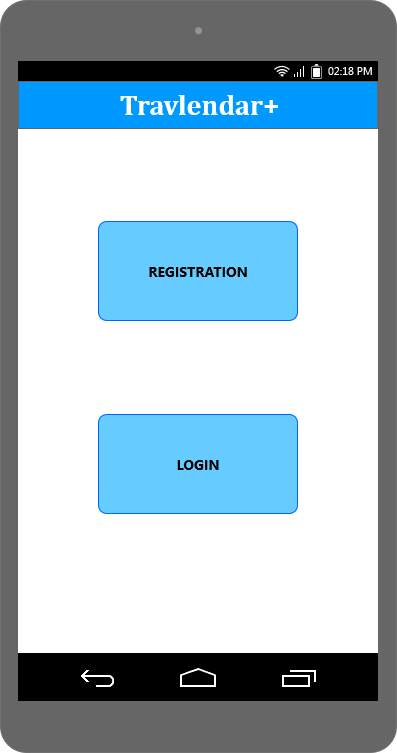
\includegraphics[scale=0.35]{mockup/app/Start/00-Start}
		\hspace{.3cm}
		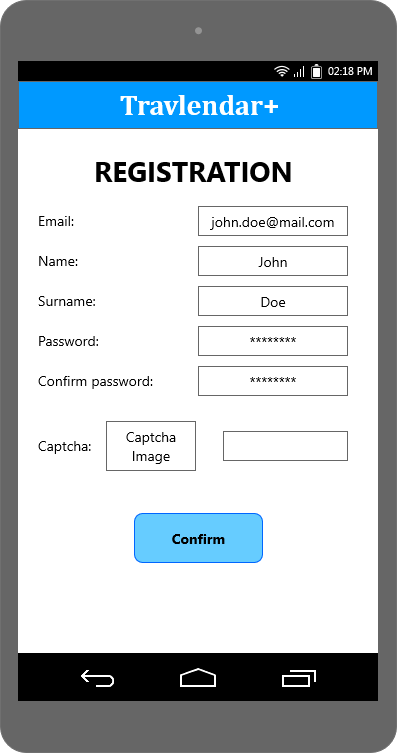
\includegraphics[scale=0.35]{mockup/app/Start/01-Register}
		\hspace{.3cm}
		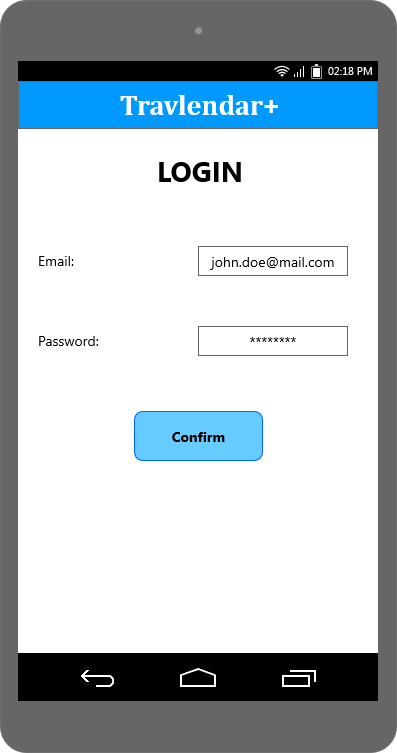
\includegraphics[scale=0.35]{mockup/app/Start/02-Login}
		\centering
		\caption{The user can register and log into the system.}
	\end{figure}
	
	\begin{figure}[H]
		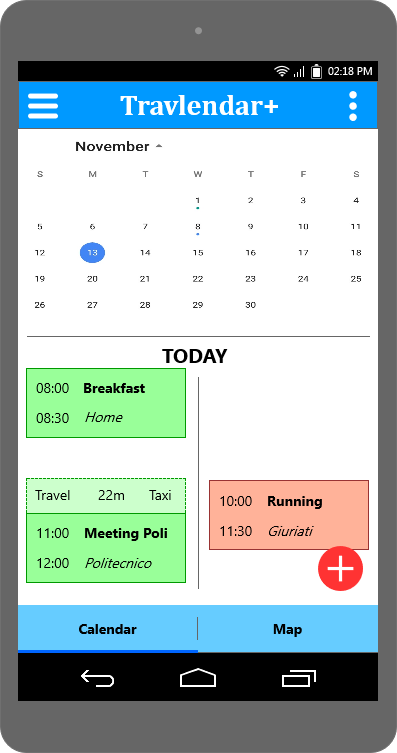
\includegraphics[scale=0.35]{mockup/app/Calendar/00-Calendar}
		\hspace{.3cm}
		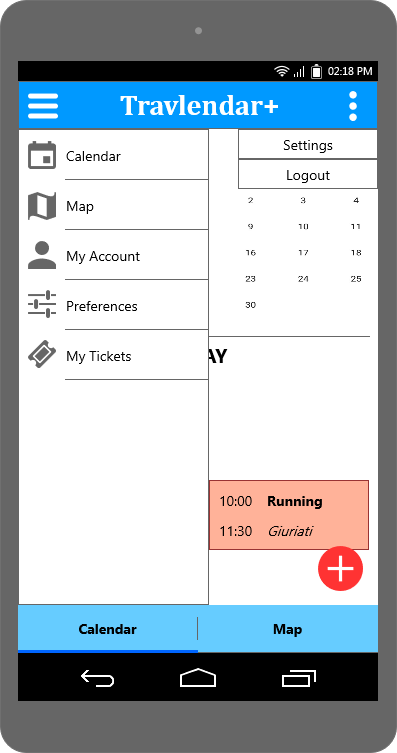
\includegraphics[scale=0.35]{mockup/app/03-Nav_Menu}
		\hspace{.3cm}
		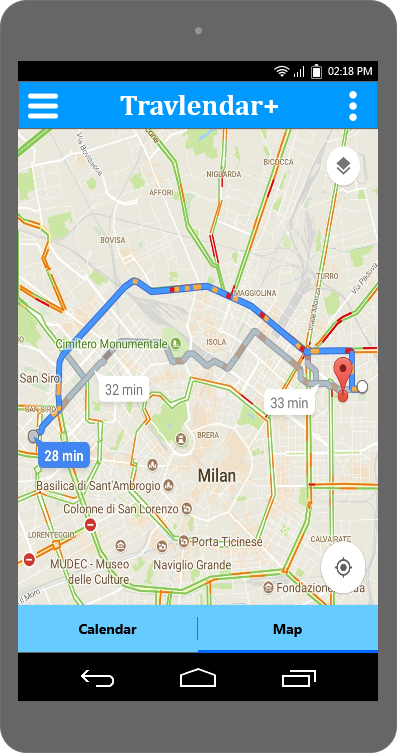
\includegraphics[scale=0.35]{mockup/app/04-Map}
		\centering
		\caption{The main screens of the application.}
	\end{figure}

	\begin{figure}[H]
		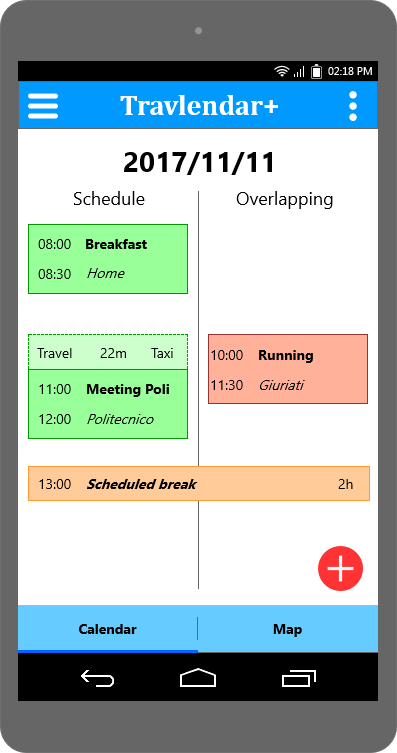
\includegraphics[scale=0.35]{mockup/app/Calendar/Schedule/00-Schedule}
		\hspace{.3cm}
		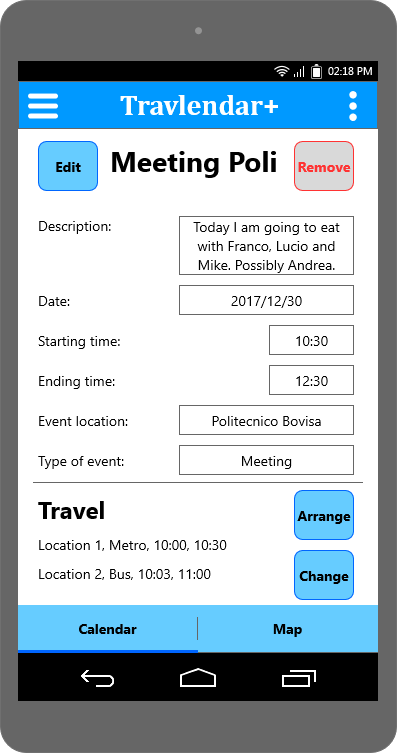
\includegraphics[scale=0.35]{mockup/app/Calendar/Schedule/01-View_Event}
		\centering 
		\caption{The user can see his schedule and view its events.}
	\end{figure}
	
	\begin{figure}[H]
		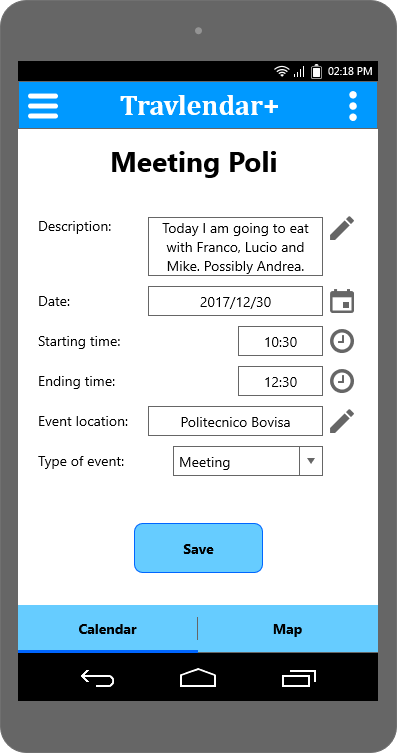
\includegraphics[scale=0.35]{mockup/app/Calendar/Schedule/02-Edit_Event}
		\hspace{.3cm}
		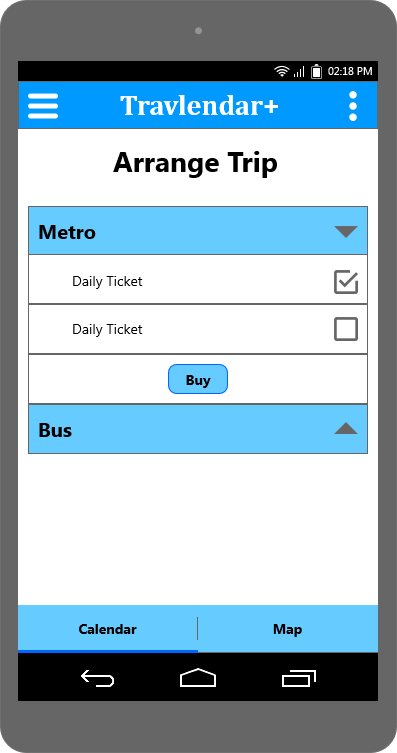
\includegraphics[scale=0.35]{mockup/app/Calendar/Schedule/03-Arrange_Trip}
		\centering 
		\caption{The user can edit and arrange its trip.}
	\end{figure}
	
	\begin{figure}[H]
		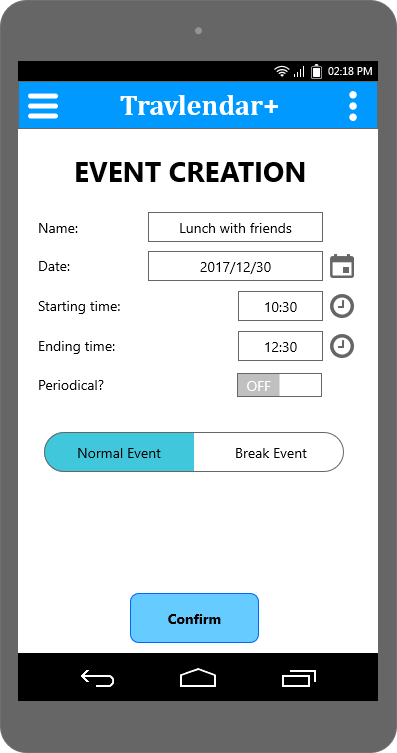
\includegraphics[scale=0.35]{mockup/app/Calendar/Create_Event/00-Create_Event}
		\hspace{.3cm}
		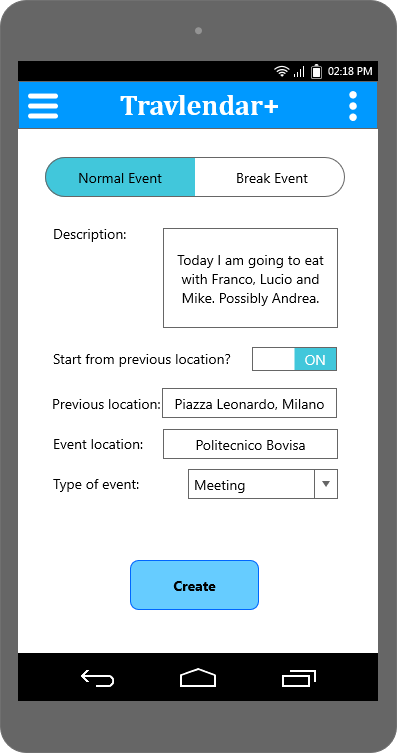
\includegraphics[scale=0.35]{mockup/app/Calendar/Create_Event/01-Create_Normal_Event}
		\hspace{.3cm}
		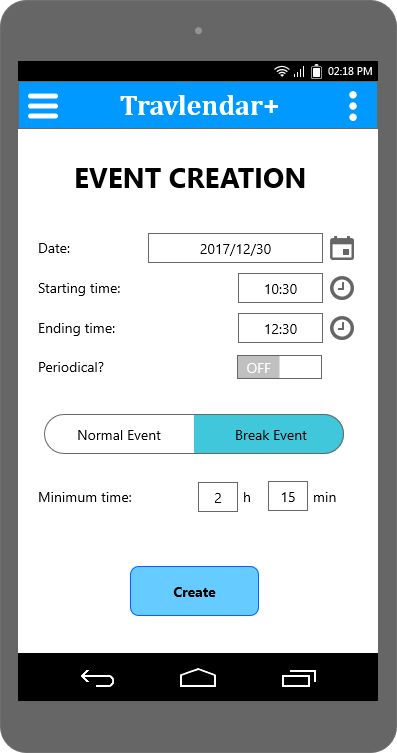
\includegraphics[scale=0.35]{mockup/app/Calendar/Create_Event/02-Create_Break_Event}
		\centering 
		\caption{The user can create an event, specifying if it's a break event or a normal one.}
	\end{figure}
	
	\begin{figure}[H]
		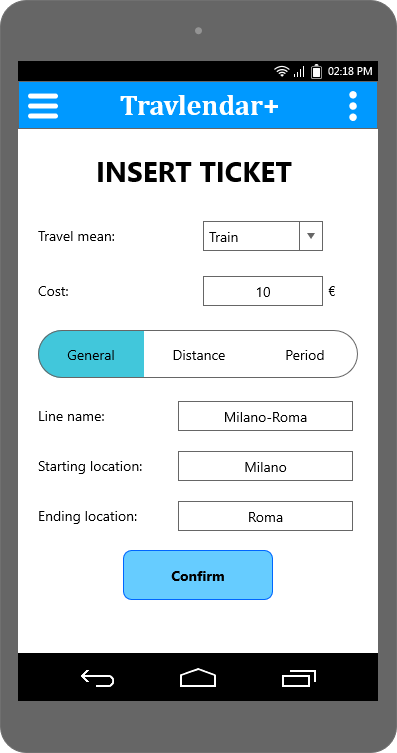
\includegraphics[scale=0.35]{mockup/app/My_Tickets/Add_Ticket/01-Add_General_Ticket}
		\hspace{.3cm}
		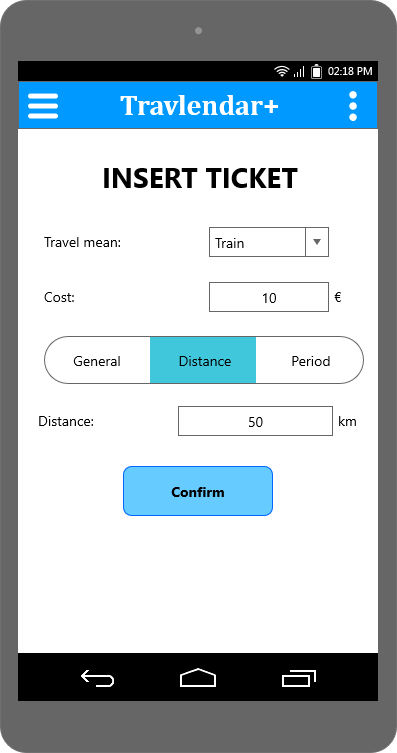
\includegraphics[scale=0.35]{mockup/app/My_Tickets/Add_Ticket/02-Add_Distance_Ticket}
		\hspace{.3cm}
		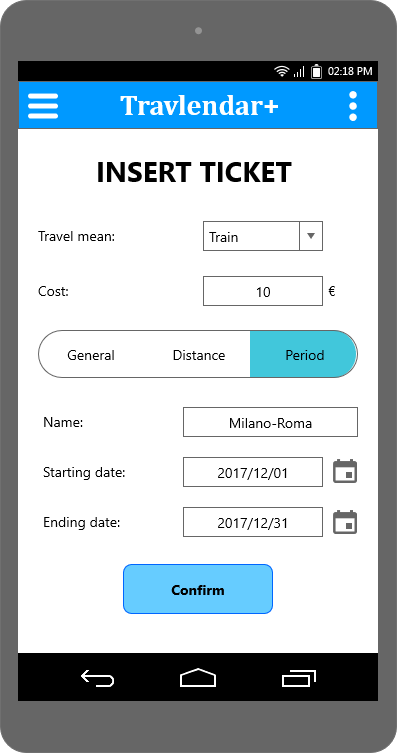
\includegraphics[scale=0.35]{mockup/app/My_Tickets/Add_Ticket/03-Add_Period_Ticket}
		\centering 
		\caption{The user can handle his tickets.}
	\end{figure}
	
	\begin{figure}[H]
		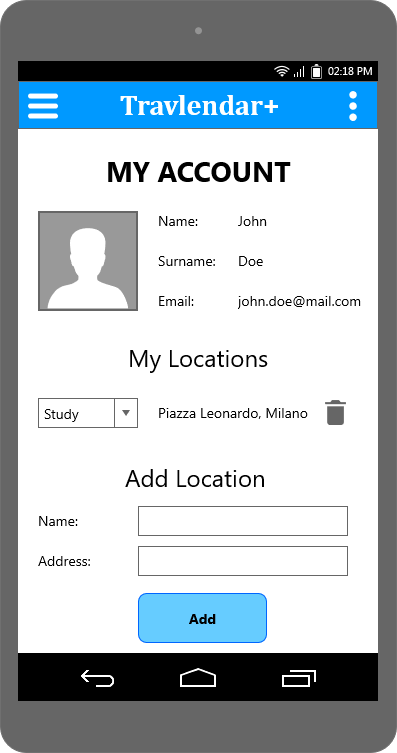
\includegraphics[scale=0.35]{mockup/app/05-My_Account}
		\hspace{.3cm}
		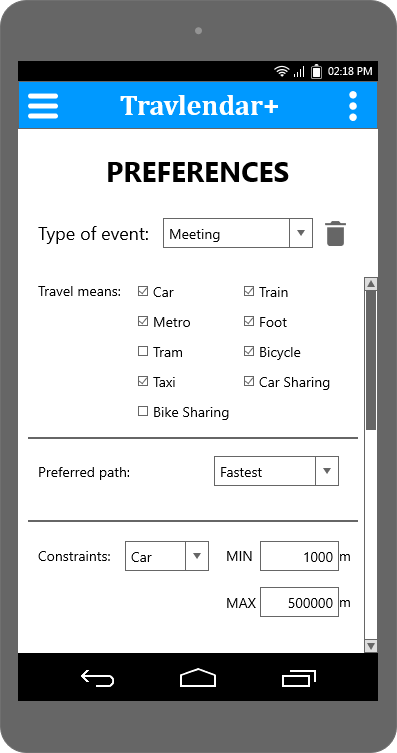
\includegraphics[scale=0.35]{mockup/app/06-Preferences}
		\hspace{.3cm}
		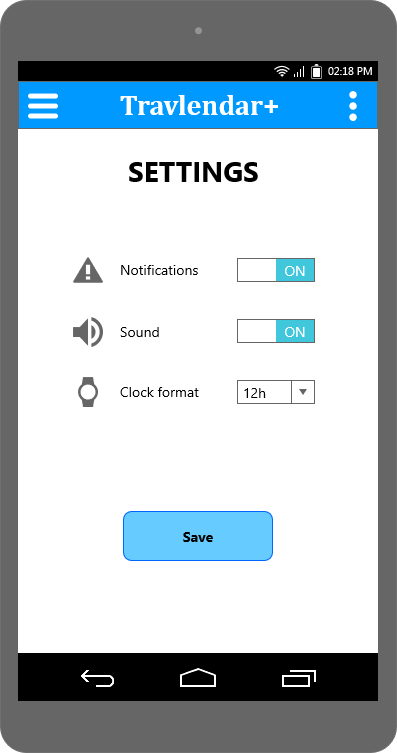
\includegraphics[scale=0.35]{mockup/app/08-Settings}
		\centering 
		\caption{The user can modify his preferences and the system settings.}
	\end{figure}
	
	\begin{figure}[H]
		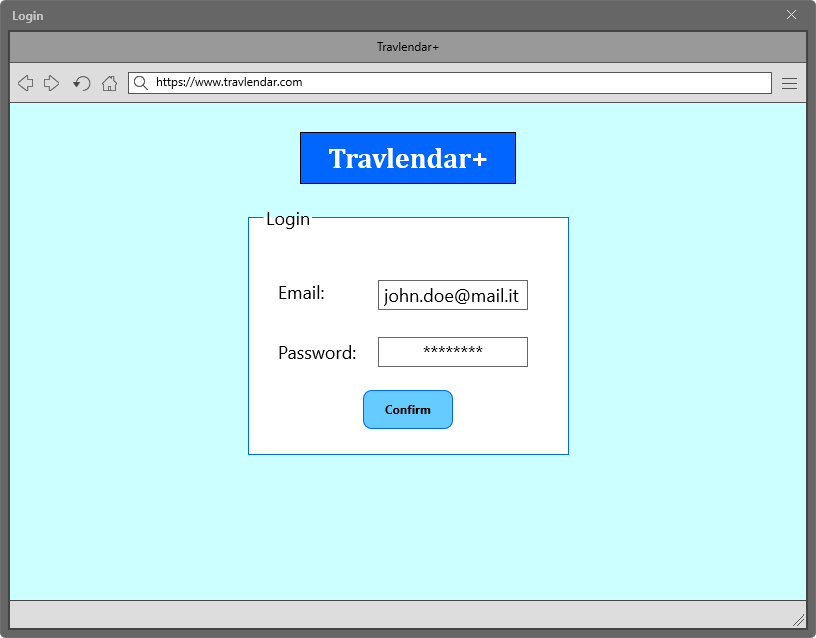
\includegraphics[scale=0.35]{mockup/web/01-Login}
		\centering
		\caption{Web browser login view.}
	\end{figure}
	\begin{figure}[H]
		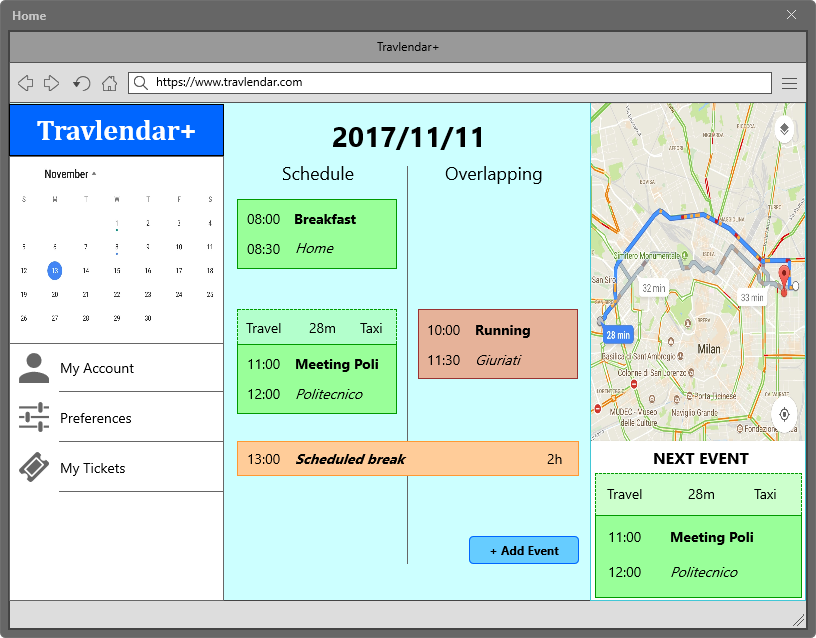
\includegraphics[scale=0.35]{mockup/web/02-Home}
		\centering
		\caption{Web browser home view.}
	\end{figure}
	\begin{figure}[H]
		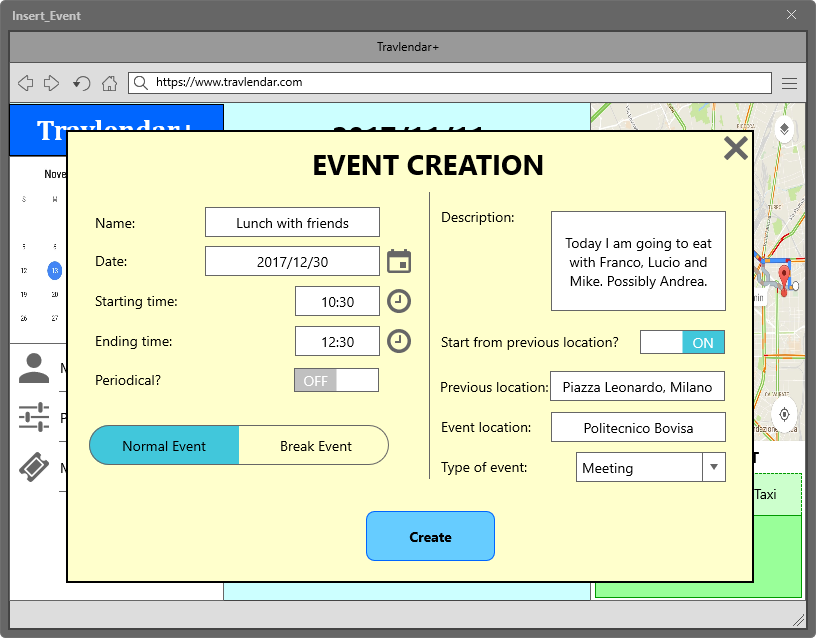
\includegraphics[scale=0.35]{mockup/web/03-Insert_Event}
		\centering
		\caption{Web browser event creation view.}
	\end{figure}

\section{UX diagrams}
\label{subsect:UX diagrams}
	The following UX diagram provides additional information about the user interface.
Screens are modeled using \textit{\textless\textless screen\textgreater\textgreater} stereotyped classes, while input forms and screen compartments are represented with separate \textit{\textless\textless input form\textgreater\textgreater} and \textit{\textless\textless screen compartment\textgreater\textgreater}
stereotyped classes.
	\begin{figure}[H]
		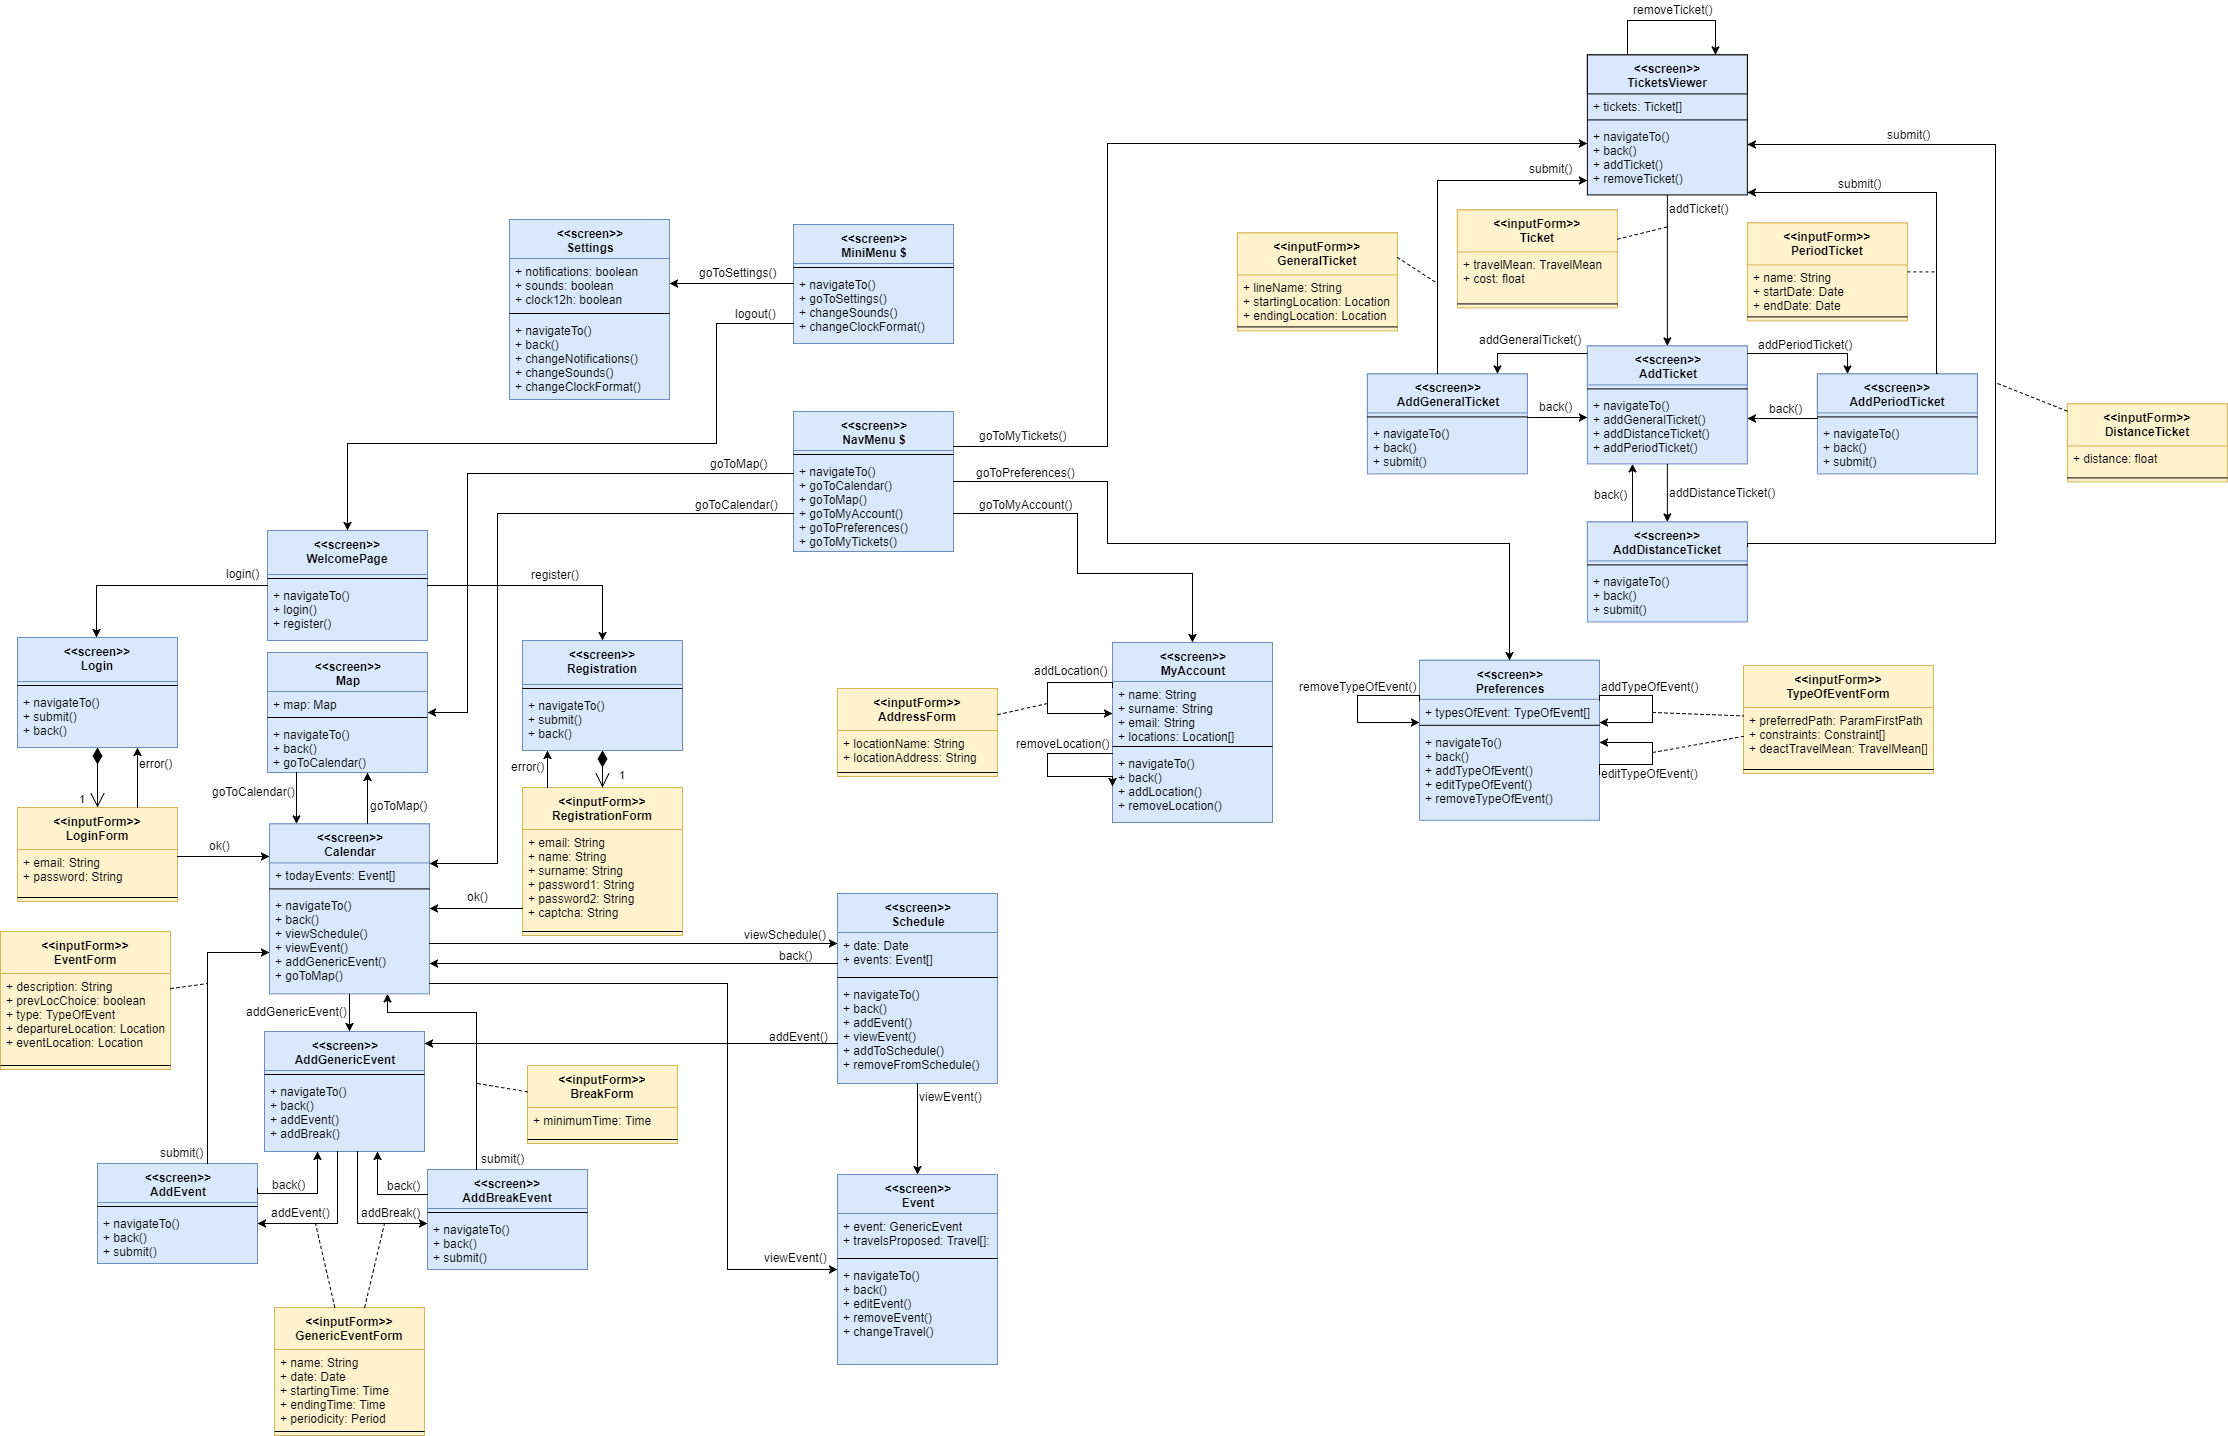
\includegraphics[width=\textheight, angle=90]{ux_diagram}
		\centering
	\end{figure}
	
\section{BCE diagram}
\label{subsect:BCE diagram}
	\begin{figure}[H]
	\vspace*{-55px}
		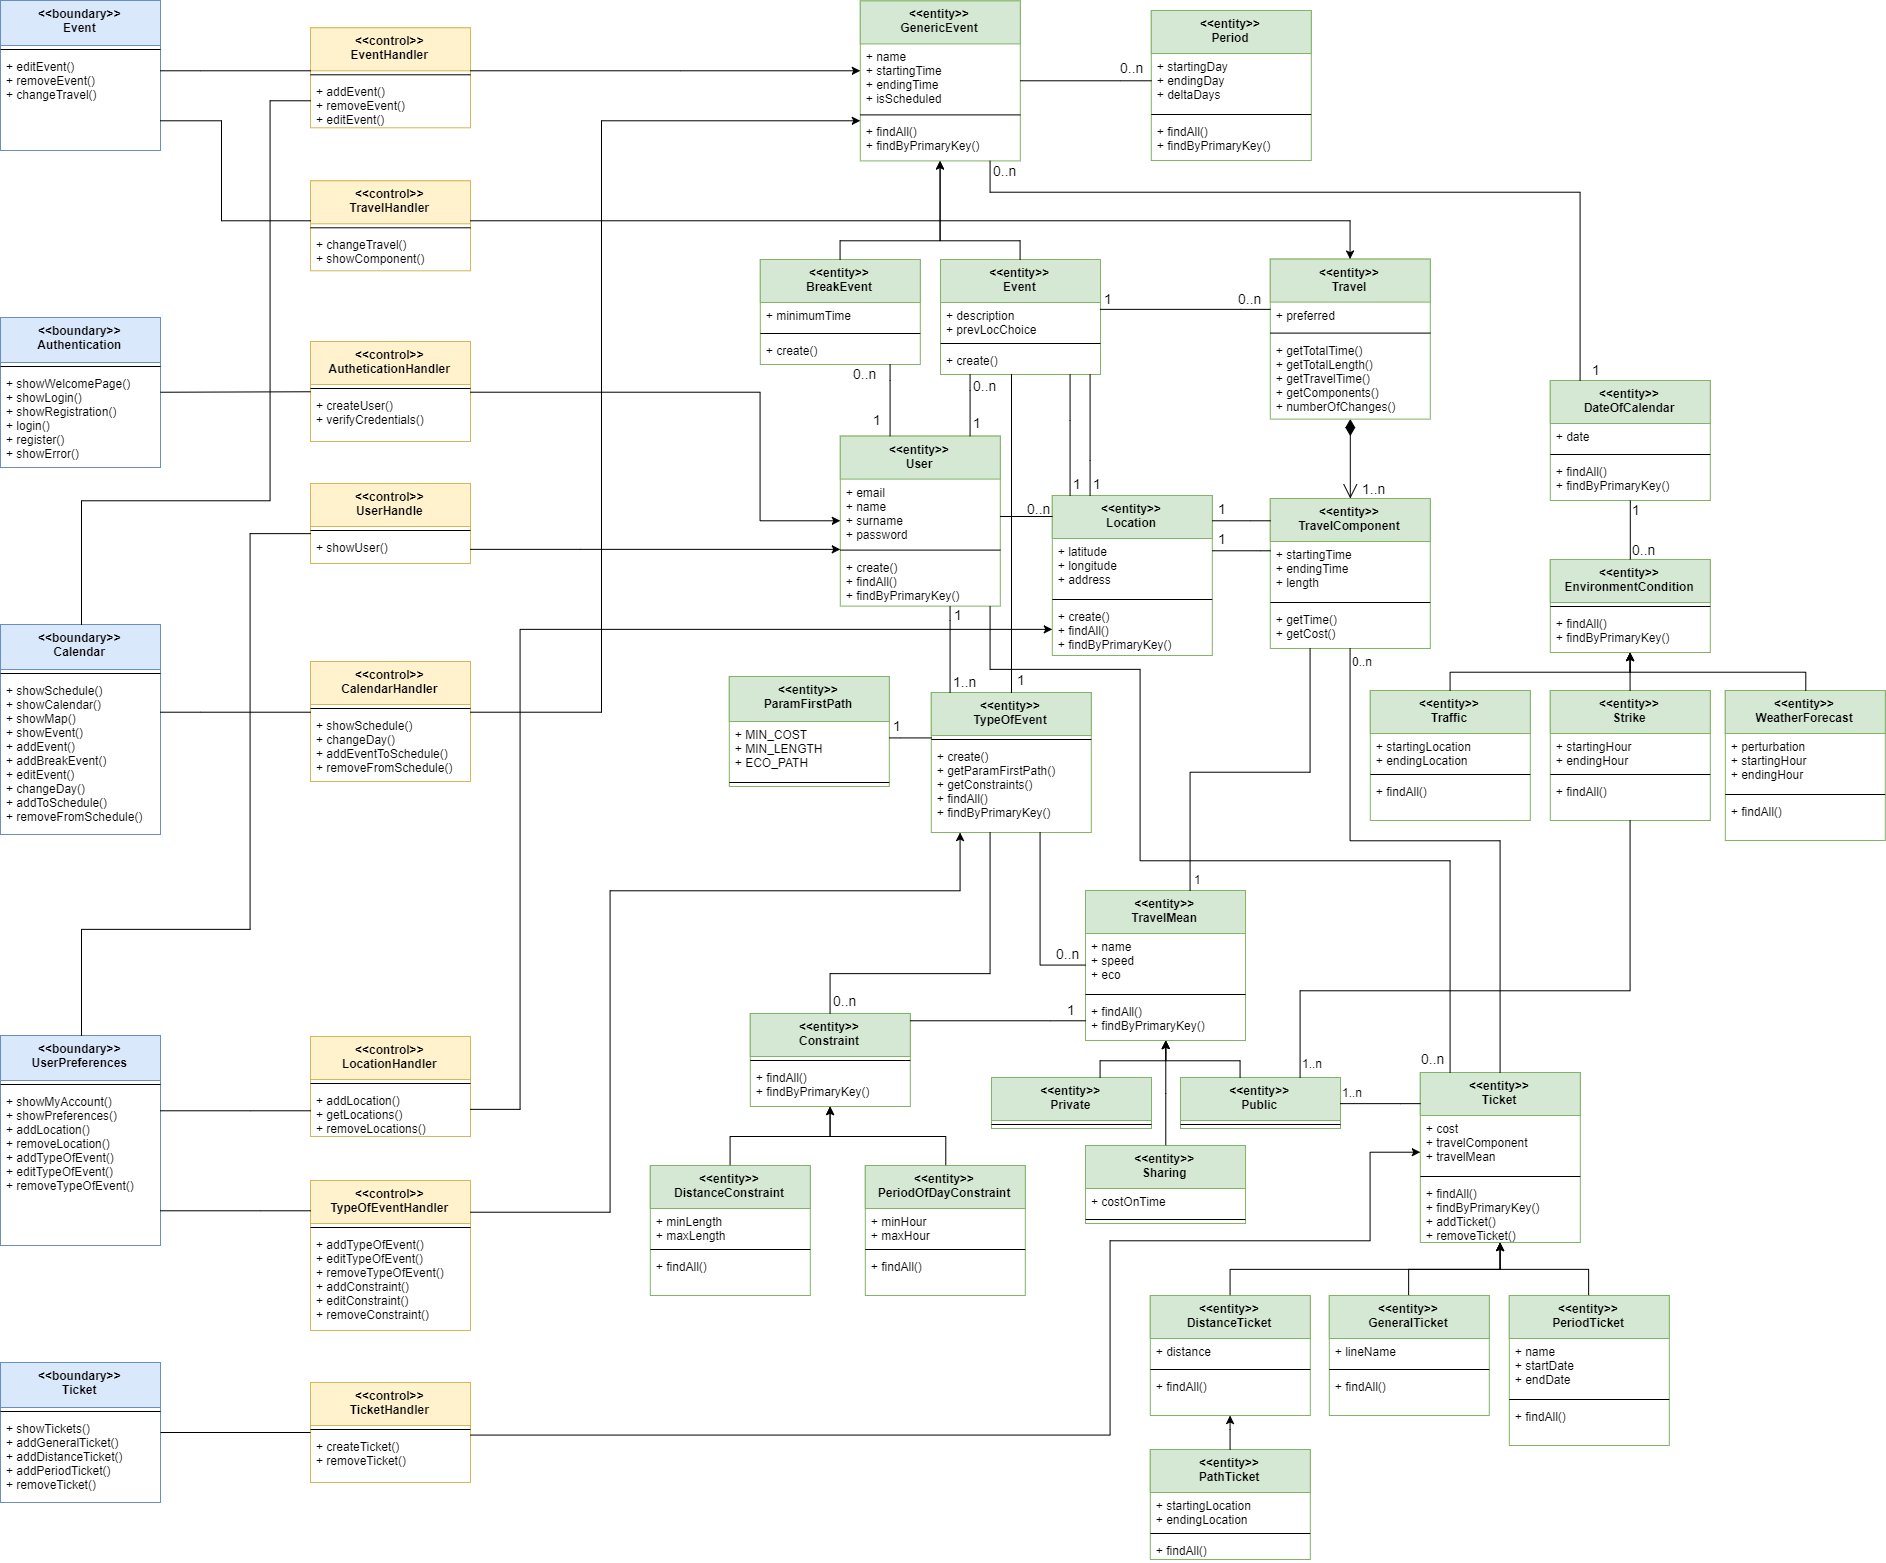
\includegraphics[width=\textheight, height=\textwidth, angle=90]{bce_diagram}
		\centering
	\end{figure}
	Given an adopted MVC pattern design, the following diagrams present a plausible representation of the system, separating internal representations of information from information presentation. \textit{Boundaries} are objects, such as user interfaces, that interface with system actors; \textit{Controls} are objects that manage interactions between
boundaries and entities implementing the application logic required to process
user requests; \textit{Entities} are used to model access to data.